\documentclass{article}

\usepackage[utf8]{inputenc}
\usepackage{geometry}
\usepackage{graphicx}
\usepackage{titling}
\usepackage{fancyhdr}
\usepackage{cmbright}

\geometry{
	a4paper,
	total={170mm, 257mm},
	left=20mm,
	top=20mm
}


\title{Chapter 4: Vehicle 4 - Values and Special Tastes}
\author{Fharook Shaik}
\date{26 November 2024}

\fancypagestyle{fancy}{
	\fancyhf{}
	\fancyfoot[R]{
\includegraphics[width=3cm]{images/BTULogo_englisch_grau_2x.png}}
	\fancyfoot[L]{\thedate}
	\fancyhead[L]{13869 - Braitenberg Vehicle Praktium}
	\fancyhead[R]{\theauthor}
}

\pagestyle{fancy}

\makeatletter
\renewcommand{\maketitle}{
	\thispagestyle{fancy}
	\null
	\vskip 1em
	\begin{center}
		{\LARGE \@title \par}
	\end{center}
	\vskip 3em
}
\makeatother


\begin{document}

	\maketitle

	\noindent\begin{tabular}{@{}ll}
		Student & \theauthor\\
		Professor &  Dr. Cunningham, Douglas\\
		Matrikel-Nr.: & 5014962
		 
	\end{tabular}

	\section*{Summary}
	In Chapter 4 of \textit{Vehicles: Experoments in Synthetic Phsycology}, Valentino Braitenberg introduces Vehicle 4, a new type of vehicle that builds on the behaviours of earlier models by modifying how sensors influence motors. Vehicle 4 introduces \textit{nonmonotonic} and \textit{threshold-based responses} resulting in behaviours that are more intricate and lifelike than those seen before.

	\subsection*{Vehicle 4a: Nonmonotonic Behaviour}
	The primary innovation in the vehicle 4a is the use of nonmonotonic connections between sensors and motors. Unlike earlier vehicles, where motor speed either continously increased ("the more, the more") or decreased ("the more, the less") with sensor stimulation, Vehicle 4a's motor speed increases only up to a certain point, beyond which it begins to decrease. This adjustment allows for more nuanced behaviours.

	A Vehicle 4a might navigate toward a source, a vehicle 2b would, but turn away when the stimulus becomes too strong. It might then circle back, repeating this pattern over and over, potentially forming trajectories like in figure eight. It could orbit around a source at a fixed distance, adjusting its course based on stimulus intensity. Weaker stimuli pull it closer to the source, while stronger stimuli push it away. Preferences emerge, such as liking a weak stimulus but avoiding a strong one, or vice versa. For example, it might turn away from a faint smell but destroy the source of a strong one. It may alternate between different stimuli, such as moving toward a smell, then switching to sound, and then turning away from both if the temparature changes. 
	
	These behavoiurs create an impression of "instincts", as though the vehicle is motivated by complex internal preferences or desires. However, Braitenberg reminds us that these behaviours are purely mechanical, driven by the nonmonotonic design of sensor-motor connections.
	
	\begin{figure}[h]
		\centering
		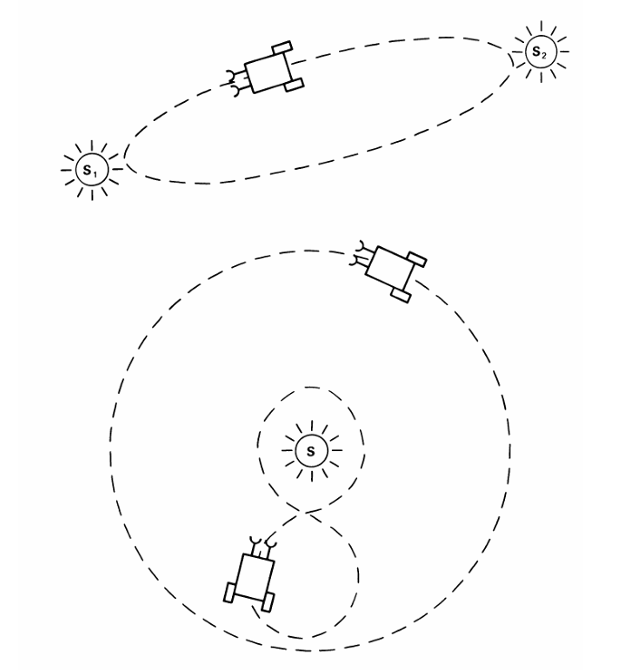
\includegraphics[scale=0.6]{images/figure_7.png}
		\caption{Vehicle 4a trajectories around and between sources}
		\label{fig:vehicle-4a}
	\end{figure}

	\subsection*{Vehicle 4b: Threshold-based Behaviour}
	Vehicle 4b builds on the idea of nonmonotonic responses by introducing **thresholds** into the system. Instead of smooth, continuous changes in motor activation, this vehicle introduces abrupt changes based on stimulus intensity.

	The motor remains inactive until the stimulus intensity crosses a specific threshold. Once this happens, the motor activates and may run at full speed or follow a smoother pattern of activation. For example, a Vehicle 4b might remain stationary in weak stimuli but suddenly start moving when the intensity exceeds the threshold. The motor may also display gradual changes within certain ranges of intensity but with sharp, abrupt shifts at specific points.

	Observers might interpret these threshold-based actions as signs of decision-making or deliberation. The vehicle appears to "ponder" over its actions, delaying movement until the stimulus becomes strong enough.This delay followed by decisive action can make the vehicle seem spontaneous and purposeful, as though it has a "will" to act.

	Braitenberg notes that these threshold-based responses are not entirely artificial. In real-world systems, friction naturally enforces thresholds, as motors must generate enough force to overcome resistance before movement begins. This adds to the realism of Vehicle 4b's behavior.

	\begin{figure}[h]
		\centering
		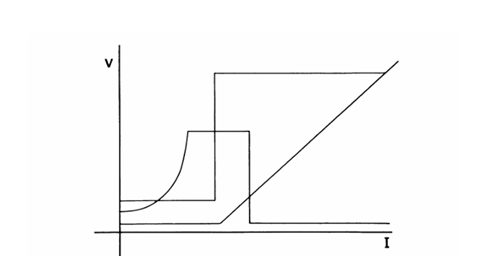
\includegraphics[scale=1]{images/figure_8.png}
		\caption{Dependence of the speed of the motor on the intensity of stimulation in Vehicle 4b}
		\label{fig:vehicle-4b}
	\end{figure}

	\subsection*{}

	Watching Vehicle 4a or 4b in action, an observer might attribute complex emotions, instincts, or decision-making to these vehicles. Vehicle 4a's orbiting or switching behaviors could suggest preferences or "special tastes," while Vehicle 4b's threshold-based responses might appear as deliberation or even free will. However, Braitenberg reminds us that these are illusions created by mechanical design, not actual knowledge or intent.


	Vehicle 4 introduces a significant leap in behavioral complexity by using nonmonotonic connections and thresholds. These innovations allow the vehicles to respond in ways that seem thoughtful and deliberate, creating behaviors that mimic instincts, preferences, and even decision-making. By combining these principles with earlier designs, Braitenberg demonstrates how simple mechanical systems can produce rich, lifelike patterns of interaction with their environment.


\end{document}